\subsection{Registrering på PDF}
I dette afsnit vises design, brugergrænseflade, implementering og test for 'Registrering på PDF' viewet. For den fulde dokumentation henvises til Arkitektur og Design dokumentationens afsnit \ref{Design-sec:PDF} Registrering på PDF.
\subsubsection{Design}
Sekvensdiagrammerne for registrering på PDF-tegning, er opdelt i tre, for at overskueliggøre flowet. \\
Det første sekvensdiagram viser, hvordan applikationen loader PDF-tegningen ind. Sekvensdiagrammet kan ses på Figur \ref{fig:LoadPDFSekvensDiagram}.
\begin{figure}[H] % (alternativt [H])
	\centering
	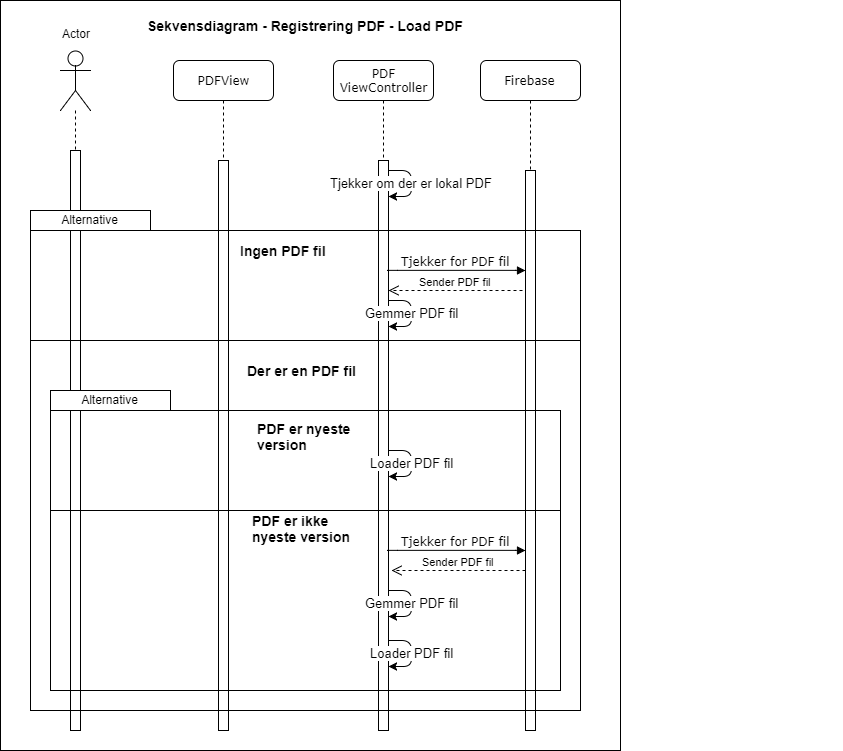
\includegraphics[height=12cm, width=15cm]{Design/Applikation/RegistrePDF/LoadPDFSekvensDiagram}
	\caption{Sekvensdiagram for Registrering på PDF - Loading af PDF, i Rambøll Tilsyn.}
	\label{fig:LoadPDFSekvensDiagram}
\end{figure}

\clearpage

Andet sekvensdiagram viser, hvordan JSON-filen bliver oprettet. Sekvensen med JSON sker direkte efter, at PDF sekvensen er overstået. Sekvensdiagrammet kan ses på Figur \ref{fig:LoadJSONSekvensDiagram}.
\begin{figure}[H] % (alternativt [H])
	\centering
	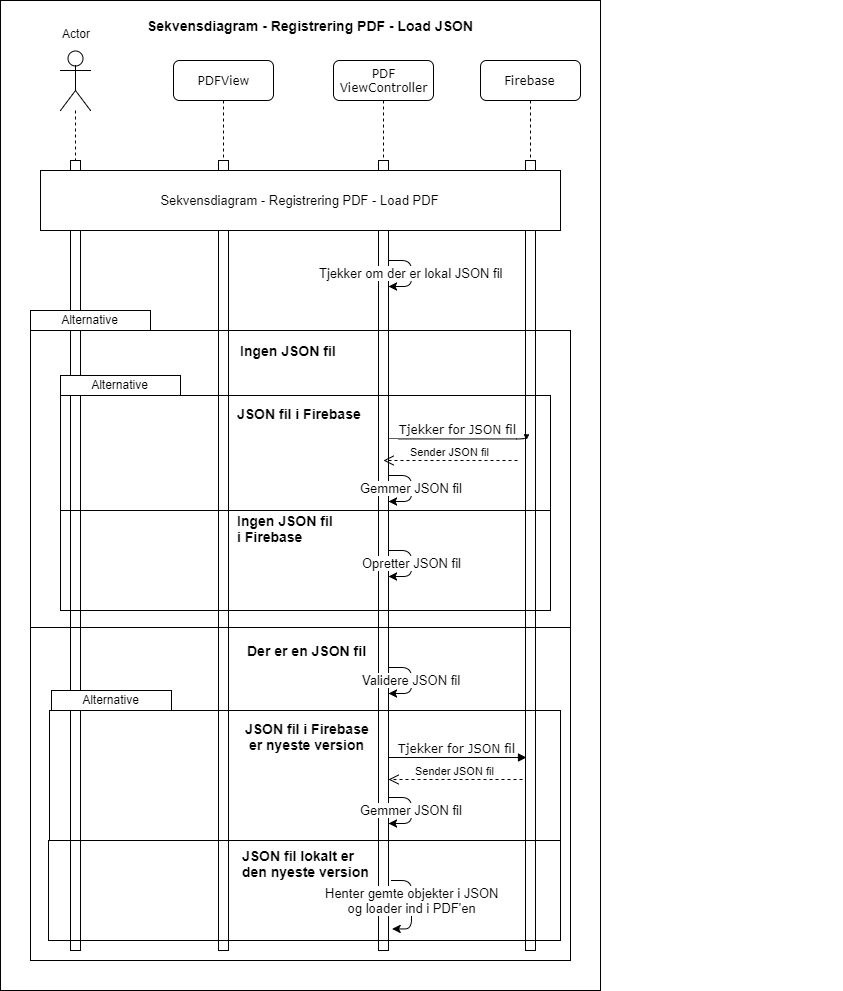
\includegraphics[height=15cm, width=15cm]{Design/Applikation/RegistrePDF/LoadJSONSekvensDiagram}
	\caption{Sekvensdiagram for Registrering på PDF - Loading af JSON, i Rambøll Tilsyn.}
	\label{fig:LoadJSONSekvensDiagram}
\end{figure}

\clearpage

Sidste sekvensdiagram for 'Registrering på PDF', sker i forlængelse, af først Loading af PDF og Load JSON og viser, hvordan systemet agerer, når brugeren interagere med applikationen i forbindelse med oprettelse af objekter på PDF-tegningen. Sekvensdiagrammet for dette, kan ses på Figur \ref{fig:RegistrerObjekterSekvensDiagram}.
\begin{figure}[H] % (alternativt [H])
	\centering
	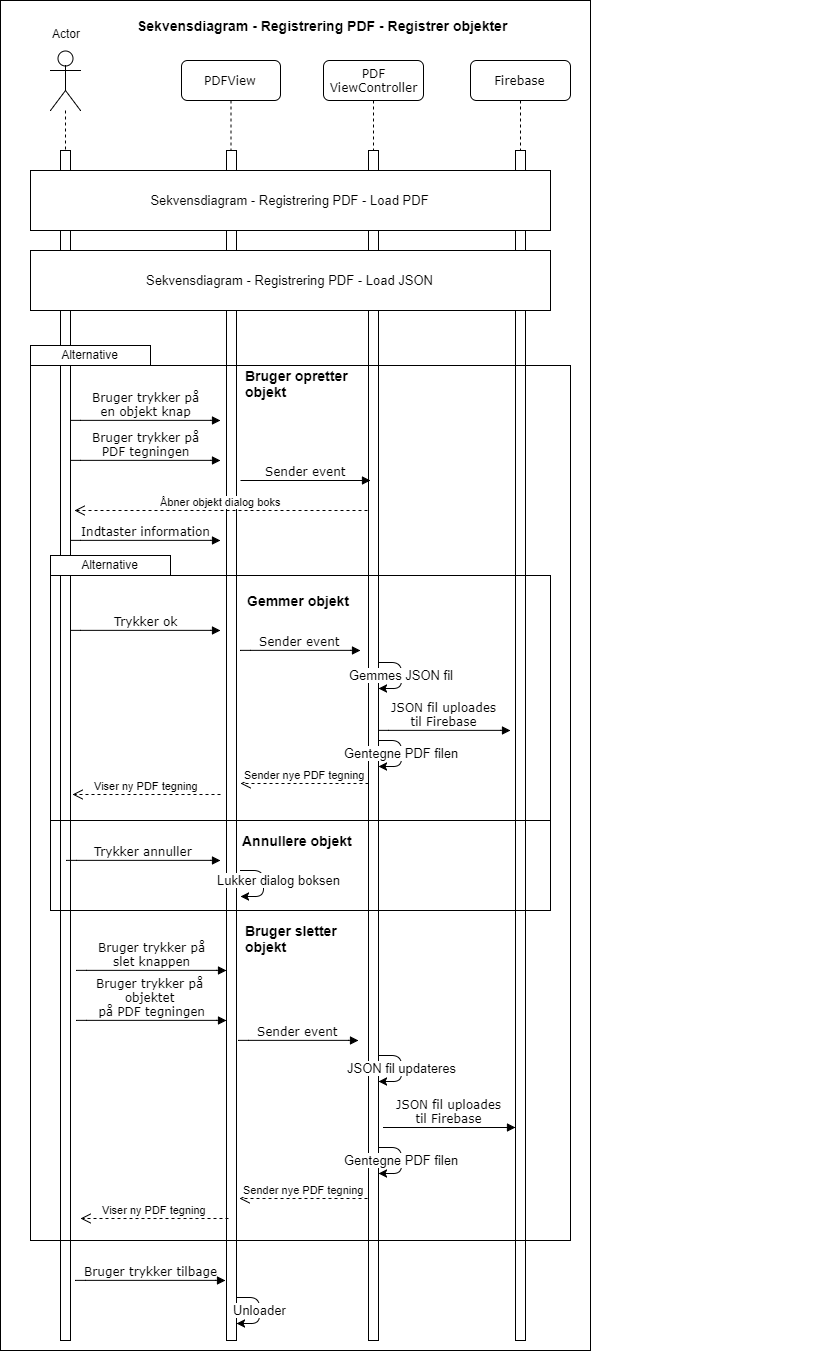
\includegraphics[height=18cm, width=15cm]{Design/Applikation/RegistrePDF/RegistrerObjekterSekvensDiagram}
	\caption{Sekvensdiagram for Registrering på PDF - Registrer på PDF, i Rambøll Tilsyn.}
	\label{fig:RegistrerObjekterSekvensDiagram}
\end{figure}

\clearpage

\subsubsection{Grafisk brugergrænseflade}
Grænsefladen for 'Registrer på PDF' viewet, som ses på Figur \ref{fig:RegistrerObjekterView} består af to views. 
Det øverste view viser PDF'en, som tilhører projektet. \\
Det nederste view indeholder knapper, som brugeren kan interagere med. Der er seks forskellige knapper: \\
De første to er frem og tilbage, hvor brugeren kan bladre mellem de forskellige sider i PDF'en. De næste tre knapper, er de symboler, som brugeren kan tegne med på PDF'en ved at trykke på knappen og derefter det sted på PDF'en, brugeren ønsker. \\
Sidste knap er en liste-knap. Her har brugeren mulighed for at afslutte sin registrering.
\begin{figure}[H] % (alternativt [H])
	\centering
	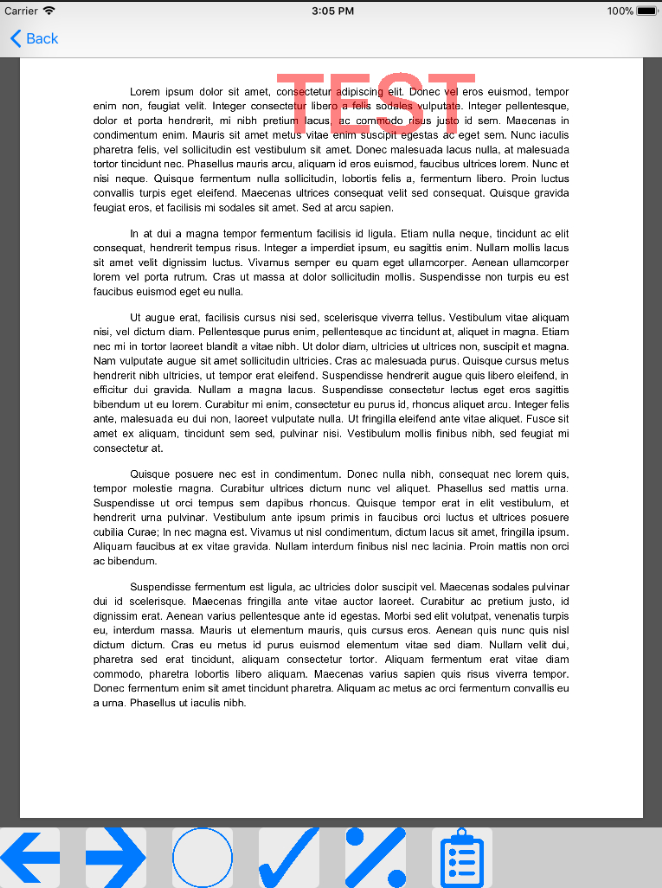
\includegraphics[height=12cm, width=10cm]{Design/Applikation/RegistrePDF/PDF}
	\caption{'Registrer på PDF' viewet, som det er implementeret i Rambøll Tilsyn.}
	\label{fig:RegistrerObjekterView}
\end{figure}

\subsubsection{Implementering}
Når der navigeres ind i 'Registrering på PDF' viewet, loades PDF'en fra Firebase og gemmes lokalt. Den loades herefter ind i viewet. Efterfølgende oprettes et UIView, hvori symbol-knapperne oprettes. Når begge dele er oprettet og loadet, hentes information fra den JSON fil der blev hentet i 'Project List' viewet, og så tegnes de objekter, som er gemt i PDF'en. \\
Når disse er tegnet, vises PDF'en for brugeren. \\
For en mere deltajeret beskrivelse af implementeringen og kode snips, henvises til Arkitektur og Design dokumentations afsnit \ref{Design-sec:PDF} Registrering på PDF.


\clearpage